\apendice{Manual de especificación de diseño}
En esta sección, se detallan los planos y el diseño arquitectónico correspondientes con el desarrollo del prototipo.
\section{Planos}
En esta sección, se incluyen los planos del prototipo. 

En la figura \ref{fig:Vista esquemática prototipo.}, se puede observar una vista esquemática del circuito del prototipo creada mediante el programa tinkercad. 
\begin{figure}
    \centering
    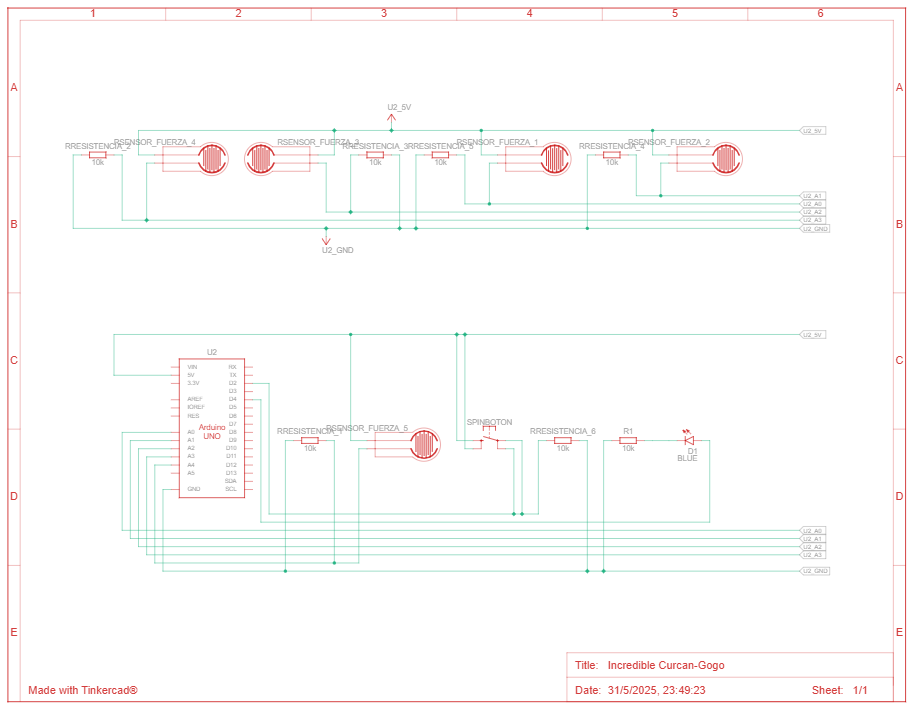
\includegraphics[width=0.8\linewidth]{img/Vista esquematica prototipo.png}
    \caption{Vista esquemática prototipo. Fuente propia}
    \label{fig:Vista esquemática prototipo.}
\end{figure}

En la figura \ref{fig:Circuito del prototipo}, se puede observar una vista del circuito del prototipo creada mediante el programa tinkercad. 
\begin{figure}
    \centering
    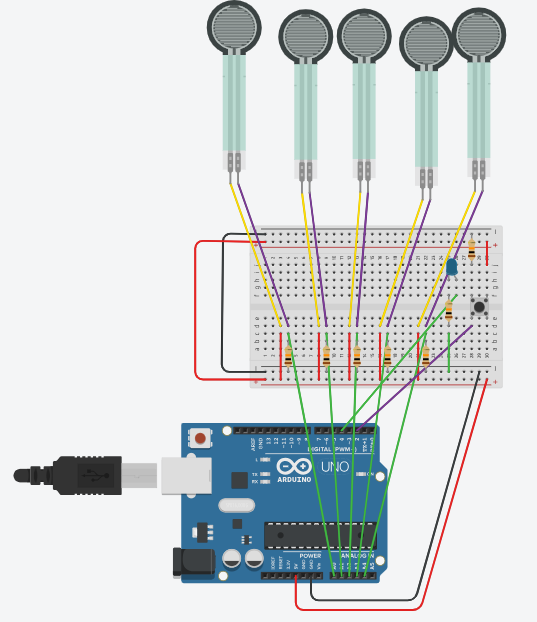
\includegraphics[width=0.5\linewidth]{img/Circuito.png}
    \caption{Circuito del prototipo. Fuente propia}
    \label{fig:Circuito del prototipo}
\end{figure}

Con estas dos figuras se pueden observar los componentes utilizados de una manera gráfica y el modo de necesario para realizar las conexiones de forma correcta.

\section{Diseño arquitectónico}

En la figura \ref{fig:Diagrama_flujo_arduino}, se puede observar un diagrama de flujo del proceso de lectura de los valores recogidos por los sensores de la placa Arduino. 

\begin{figure}
    \centering
    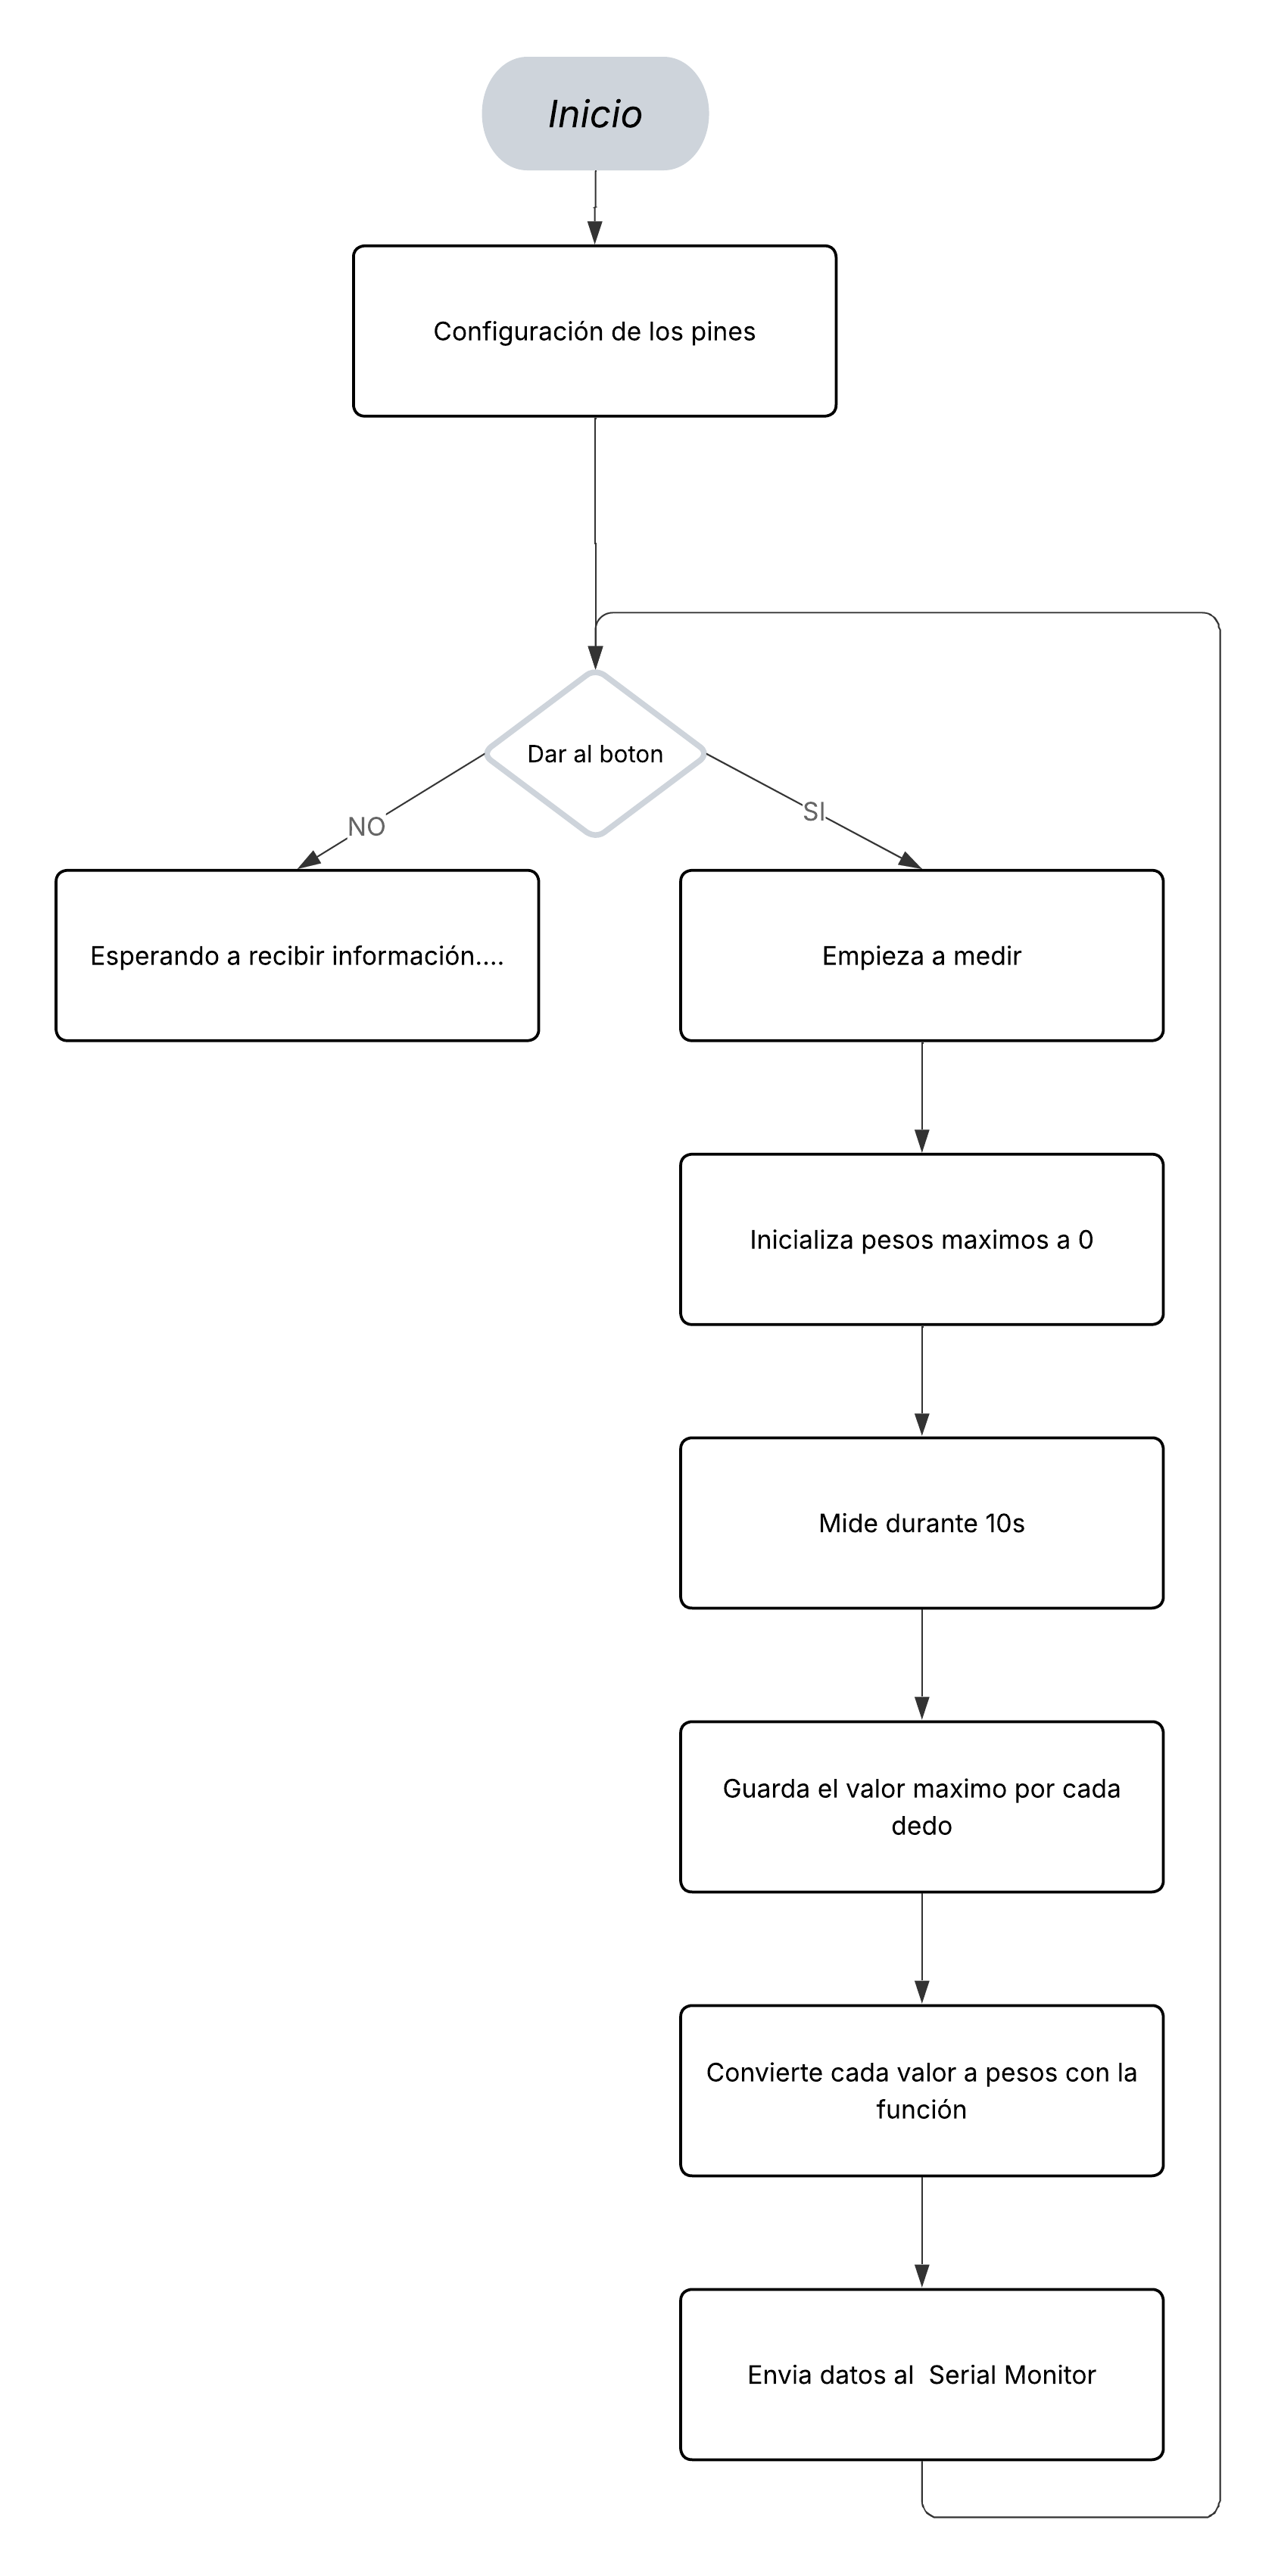
\includegraphics[width=0.5\linewidth]{img/Diagrama_flujo_arduino.png}
    \caption{Diagrama flujo de la placa Arduino. Fuente propia}
    \label{fig:Diagrama_flujo_arduino}
\end{figure}

En la figura , se puede observar un diagrama de clases que representan todas las clases definidas el archivo app.py. Este diagrama facilita la comprensión del código al mostrar la relaciones entre clases, así como los métodos contenidos en cada una de ellas.